Here, we are given a sentence $\mathcal{S}$ as a $N$-length sequence of tokens, $\mathcal{S} = \langle w_1, w_2 \ldots w_N \rangle$ and a span $\langle s, e\rangle$ where $s \in [1, N]$ is the \textit{start} index, $e \in [1, N]$ is the \textit{end} index. The goal is to output a label $t$ for the span such that $t \in \mathcal{T}$, where $\mathcal{T}$ is the set of all entity types.

This is modeled as the reverse of QA model for NER described in Section \ref{sec:question_answering}. For every gold entity mention (E.g. \textit{United States}) in a training set sentence, \textit{Emily}[\texttt{PERSON}] \textit{lives in United States}[\texttt{LOCATION}], we form a sample input, \textit{Emily lives in United States. What is United States?} The sentence is fed to a BERT model where we do sequence classification. The pooled sequence embedding returned by BERT is fed to a fully connected layer and converted to a probability distribution over possible entity types. In this example, the model is expected to assign maximum probability to \texttt{LOCATION}. Figure \ref{fig:span_classification} shows our span classification setup.

\begin{figure}[h!]
    \centering
    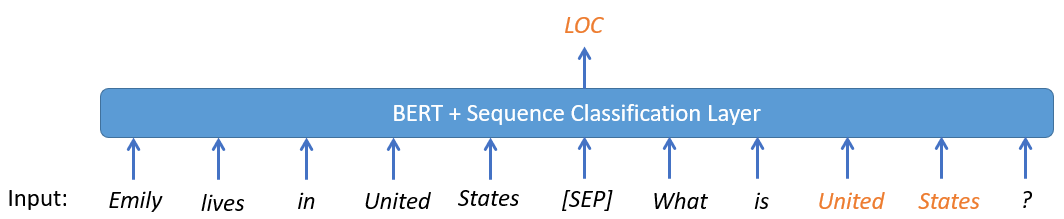
\includegraphics[width=\linewidth]{../thesis/span_classification}
    \caption{Span Classification Setup (colored tokens depict the entity mention in question with expected output entity label)}
    \label{fig:span_classification}
\end{figure}

\subsection{Pipeline}
Both the models can be trained independently. The pipeline structure comes during the inference time. Here, every unlabeled sentence is first passed through Span Detector and for each output span, we convert to an input sample for Span Classifier.

\subsection{Salient Features}

\begin{itemize}
    \item Compared to sequence labeling and question answering approach, this span-based approach has more representative power. This is because here we have two BERT models each working on their own sub-tasks and contributing towards better NER while the other approaches just have a single model.
    
    \item Even though we are training two BERT models, they can be trained independently, in parallel. Only at inference time, we need to maintain the sequential nature.
    
    \item If we have $T$ entities of interest, then standard question answering approach creates $T$ samples for each input sentence both at train and inference time. Considering that each sentence on an average has much lesser than $T$ entity mentions, there is a lot of redundancy in this approach. 
    
    \item Our span-based approach removes QA model redundancy even though inherently we have a QA-based setup. Span Detector only sees an input sentence once and identifies all mention spans. The span classifier will work on only these identified mention spans and classify them into an entity type.
    
    \item Nevertheless, our approach has a pipeline-based structure and hence errors made by span detector propagate to the classifier. Sequence labeling and question answering approaches do not face this concern. 
    
    \item Our span-based approach shows the effectiveness of \textit{reverse question answering}. For a sentence, \textit{Emily lives in United States}, rather than asking a question of the form, \textit{"What is the \texttt{Person} mentioned in the text?"}, we ask, \textit{"What is \texttt{Emily}?"}. This opens up prospects for more intuitive forms of approaching NER, taking us closer to human understanding and interpretations.
    
    \item Comparable and even improved performance of this span-based approach compared to the general QA NER setup (results in Table \ref{tab:res_span}) shows that boundary detection of mentions has less correlation with the entity type it belongs to.
\end{itemize}

\begin{table*}[h!]
\centering
\begin{tabular}{|c|c|c|c|c|}\hline
	\textbf{} & \textbf{BioNLP13CG} & \textbf{JNLPBA} & \textbf{CoNLL 2003}\\\hline
	\texttt{Span Detection} & 90.12 & 78.35 & 95.23\\\hline
	\texttt{Span Classification} & 94.06 & 95.08 & 94.50\\\hline
	\texttt{Pipeline} & 85.89 & \textbf{75.01} & \textbf{91.64}\\\hline
	\texttt{BERT-QA} & \textbf{86.45} & 74.81 & 91.17\\\hline
	\end{tabular}
    \caption{Results: Span Pipeline (Test set Micro-F1 in \%)}
    \label{tab:res_span}
\end{table*}
